\documentclass[tikz,border=10pt]{standalone}
\usepackage{tikz}
\usetikzlibrary{arrows.meta,decorations.pathmorphing,calc}

\begin{document}
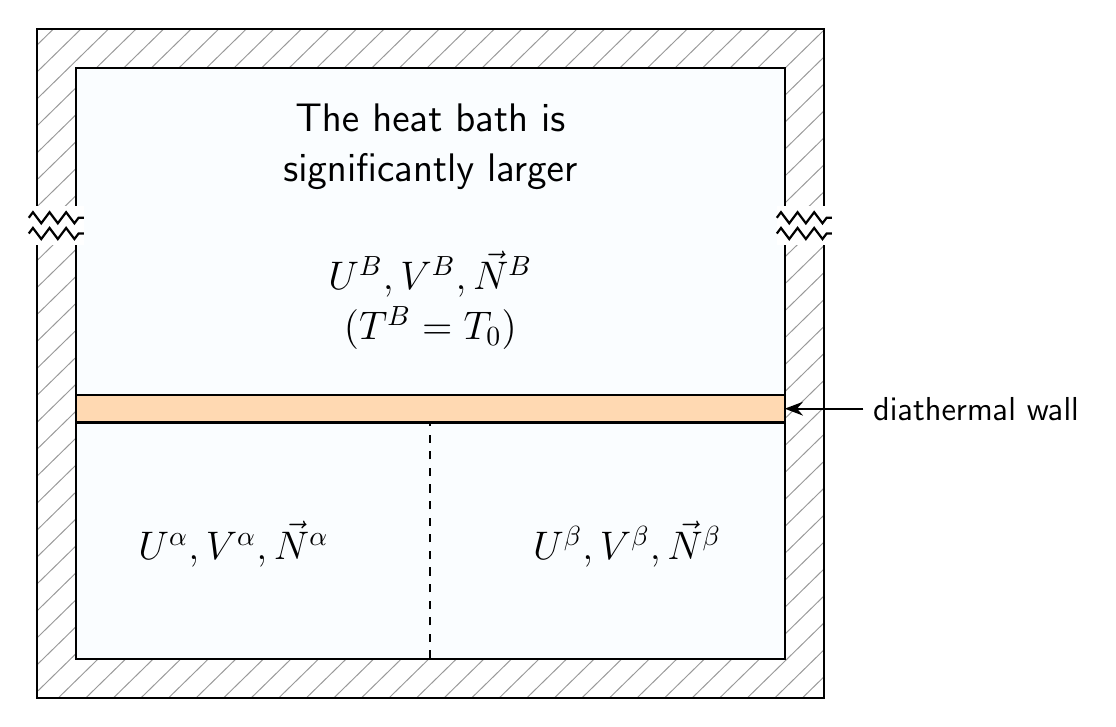
\begin{tikzpicture}
    % --- Dimensions ---
    \def\TotalW{10}       % Total Width
    \def\TotalH{8.5}      % Total Visual Height
    \def\WallThick{0.5}   % Thickness of the insulation
    \def\DiaH{0.35}       % Thickness of the diathermal wall
    \def\SplitY{3.5}      % Y-position of the separation
    \def\BreakY{6.0}      % Y-position of the visual "break"

    % --- Styles ---
    \tikzset{
        gas style/.style={
            fill=cyan!2,
            draw=black,
            thick
        },
        diathermal style/.style={
            fill=orange!30,
            draw=black,
            thick
        },
        break line/.style={
            thick,
            decorate,
            decoration={zigzag, amplitude=2pt, segment length=6pt}
        },
        math text/.style={font=\Large},
        label text/.style={font=\sffamily\Large, align=center}
    }

    % =========================================================
    % 1. INSULATION HATCH (clip to OUTER box only)
    %    Interior will be masked by the gas regions you draw later.
    % =========================================================
    \begin{scope}
      \clip (0,0) rectangle (\TotalW,\TotalH);

      \def\HatchStep{0.35} % smaller = denser
      \foreach \t in {-80,...,140} {
        \draw[gray!80, line width=0.35pt]
          (-12+\t*\HatchStep, -12) -- (-12+\t*\HatchStep+45, 32);
      }
    \end{scope}

    % Outer border
    \draw[thick] (0,0) rectangle (\TotalW,\TotalH);

    % =========================================================
    % 2. GAS CHAMBERS (these mask the hatch in the interior)
    % =========================================================
    % Bottom Compartment (Alpha & Beta)
    \filldraw[gas style]
        (\WallThick, \WallThick) rectangle (\TotalW-\WallThick, \SplitY);

    % Top Compartment (Heat Bath)
    \filldraw[gas style]
        (\WallThick, \SplitY + \DiaH) rectangle (\TotalW-\WallThick, \TotalH-\WallThick);

    % Inner border of the cavity (gives the “ring” look)
    \draw[thick] (\WallThick,\WallThick) rectangle (\TotalW-\WallThick,\TotalH-\WallThick);

    % =========================================================
    % 3. DIATHERMAL WALL
    % =========================================================
    \filldraw[diathermal style]
        (\WallThick,\SplitY) rectangle (\TotalW-\WallThick,\SplitY+\DiaH);

    % =========================================================
    % 4. VISUAL BREAKS (zigzags)
    % =========================================================
    % --- LEFT BREAK ---
    \fill[white] (-0.1, \BreakY-0.25) rectangle (\WallThick+0.1, \BreakY+0.25);
    \draw[break line] (-0.1, \BreakY+0.1) -- (\WallThick+0.1, \BreakY+0.1);
    \draw[break line] (-0.1, \BreakY-0.1) -- (\WallThick+0.1, \BreakY-0.1);

    % Restore vertical border lines
    \draw[thick] (0, \BreakY+0.25) -- (0, \TotalH);
    \draw[thick] (0, 0) -- (0, \BreakY-0.25);
    \draw[thick] (\WallThick, \BreakY+0.25) -- (\WallThick, \TotalH-\WallThick);
    \draw[thick] (\WallThick, \WallThick) -- (\WallThick, \BreakY-0.25);

    % --- RIGHT BREAK ---
    \fill[white] (\TotalW-\WallThick-0.1, \BreakY-0.25) rectangle (\TotalW+0.1, \BreakY+0.25);
    \draw[break line] (\TotalW-\WallThick-0.1, \BreakY+0.1) -- (\TotalW+0.1, \BreakY+0.1);
    \draw[break line] (\TotalW-\WallThick-0.1, \BreakY-0.1) -- (\TotalW+0.1, \BreakY-0.1);

    % Restore vertical border lines
    \draw[thick] (\TotalW, \BreakY+0.25) -- (\TotalW, \TotalH);
    \draw[thick] (\TotalW, 0) -- (\TotalW, \BreakY-0.25);
    \draw[thick] (\TotalW-\WallThick, \BreakY+0.25) -- (\TotalW-\WallThick, \TotalH-\WallThick);
    \draw[thick] (\TotalW-\WallThick, \WallThick) -- (\TotalW-\WallThick, \BreakY-0.25);

    % =========================================================
    % 5. TEXT AND ANNOTATIONS
    % =========================================================
    % Dashed Divider (Bottom)
    \draw[thick, dashed] (\TotalW/2, \WallThick) -- (\TotalW/2, \SplitY);

    % Alpha Variables
    \node[math text] at (\TotalW/4, \SplitY/2 + 0.2) {$U^\alpha, V^\alpha, \vec{N}^\alpha$};

    % Beta Variables
    \node[math text] at (3*\TotalW/4, \SplitY/2 + 0.2) {$U^\beta, V^\beta, \vec{N}^\beta$};

    % Heat Bath Text
    \node[label text] at (\TotalW/2, \TotalH - 1.5) {
        The heat bath is \\ significantly larger
    };

    % Heat Bath Variables
    \node[math text, align=center] at (\TotalW/2, \SplitY + \DiaH + 1.2) {
        $U^B, V^B, \vec{N}^B$ \\
        $(T^B = T_0)$
    };

    % Diathermal Label + Arrow
    \node[font=\sffamily\large, anchor=west] (lbl_dia)
        at (\TotalW + 0.5, \SplitY + \DiaH/2) {diathermal wall};
    \draw[->, >=Stealth, thick] (lbl_dia.west) -- (\TotalW-\WallThick, \SplitY + \DiaH/2);

\end{tikzpicture}
\end{document}